\PassOptionsToPackage{usenames,dvipsnames}{xcolor}
\documentclass[9pt,twoside,lineno]{pnas-new}
% Use the lineno option to display guide line numbers if required.

\templatetype{pnassupportinginfo}

\usepackage{natbib}
\usepackage{gensymb}
\graphicspath{{/Users/jm200/Library/CloudStorage/Dropbox/Miller Lab/github/POAR-Forecasting/Manuscript/Figures/}}
%\graphicspath{{/Users/tm9/Dropbox/github/POAR-Forecasting/Manuscript/Figures/}}
\newcommand{\tom}[2]{{\color{red}{#1}}\footnote{\textit{\color{red}{#2}}}}
\newcommand{\jacob}[2]{{\color{blue}{#1}}\footnote{\textit{\color{blue}{#2}}}}
\newcommand{\revise}[1]{{\color{Mahogany}{#1}}}
\title{Forecasting range shifts of dioecious plants under climate change}
\author{Jacob K. Moutouama, Aldo Compagnoni and Tom E.X. Miller}
\correspondingauthor{Jacob Moutouama.\\E-mail: jmoutouama@gmail.com}

\begin{document}

%% Comment out or remove this line before generating final copy for submission; this will also remove the warning re: "Consecutive odd pages found".
%\instructionspage  

\maketitle

%% Adds the main heading for the SI text. Comment out this line if you do not have any supporting information text.
\SItext


\section*{Supporting Methods}

\subsection*{A. Climatic data collection}
The general circulation models (GCMs) were selected from the Coupled Model Intercomparison Project Phase 5 (CMIP5): Model for Interdisciplinary Research on Climate (MIROC5), Australian Community Climate and Earth System Simulator (ACCESS1-3), Community Earth System Model (CESM1-BGC), Centro Euro-Mediterraneo sui Cambiamenti Climatici Climate Model (CMCC-CM).
All the GCMs were also downloaded from Chelsa \citep{sanderson2015representative}.
We evaluated future climate projections from two scenarios of representative concentration pathways (RCPs): RCP4.5, an intermediate-to-pessimistic scenario assuming a radiative forcing amounting to 4.5 $W m^{-2}$ by 2100, and RCP8.5, a pessimistic emission scenario which projects a radiative forcing of 8.5 $W m^{-2}$ by 2100 \citep{thomson2011rcp4, schwalm2020rcp8}. 

Projection data for the three 30-year periods included warmer or colder conditions than observed in our experiment, so extending our inferences to these conditions required some extrapolation. 
However, across all sites, both study years were 1-2\degree C warmer than their corresponding ``current'' (1990-2019) temperature normals (Fig. \ref{Sup:climate_normal_weather}). 
Additionally, the 2014--15 growing season was generally wetter and cooler across the study region than 2015--16 (Fig. \ref{Sup:climate_normal_weather}). 
Combined, the geographic and inter-annual replication of the common garden experiment provided good coverage of most past and future conditions throughout the study region (Fig. 1). 

\subsection*{B. Sex-specific demographic responses to climatic variation across common garden sites}
Vital rate models were fit with the same linear predictors for the expected value ($\mu$)(Eq.\ref{eq:mu}):
\begin{align}\label{eq:mu}
\begin{split}
\mu = \beta_{0} + \beta_{1}size + \beta_{2}sex + \beta_{3}pptgrow + \beta_{4}pptdorm + \beta_{5}tempgrow + \beta_{6}tempdorm \\ 
+ \beta_{7}pptgrow*sex + \beta_{8}pptdorm*sex + \beta_{9}tempgrow*sex + \beta_{10}tempdorm*sex  \\ 
+  \beta_{11}size*sex + \beta_{12}pptgrow*tempgrow + \beta_{13}pptdorm*tempdorm\\
+ \beta_{14}pptgrow*tempgrow*sex + \beta_{15}pptdorm*tempdorm*sex + \beta_{16}pptgrow^2\\
+ \beta_{17}pptdorm^2 + \beta_{18}tempgrow^2 + \beta_{19}tempdorm^2 + \beta_{20}pptgrow^2*sex  \\
+ \beta_{21}pptdorm^2*sex + \beta_{22}tempgrow^2*sex + \beta_{23}tempdorm^2*sex + \phi + \rho + \nu 
\end{split}
\end{align}
\noindent where $\beta_{0}$ is the  grand mean intercept, $\beta_{1}$ is the size dependent slopes.
$size$ was on a natural logarithm scale. 
$\beta_{2}$...$\beta_{13}$ represent the climate dependent slopes.
$\beta_{14}$...$\beta_{23}$ represent the sex-climate interaction slopes.
$pptgrow$ is the precipitation of the growing season, $tempgrow$ is the temperature of the growing season, $pptdorm$ is the precipitation of the dormant season, $tempdorm$ is the temperature of the dormant season.

All  vital rates  were  fit with second-degree polynomial functions to accommodate the possibility of hump-shaped relationships (reduced demographic performance at both extremes).
We also included two-way interactions between sex and each climate driver and between temperature and precipitation within each season, and a three-way interaction between sex, temperature, and precipitation within each season. 
We modeled survival and flowering data with a Bernoulli distribution and the growth (tiller number) with a zero-truncated Poisson inverse Gaussian distribution. 
Fertility (panicle count conditional on flowering) was modeled as zero-truncated negative binomial. 
We used generic, weakly informative priors to fit coefficients for survival, growth, flowering models ($\beta \sim N(0,\ 1.5)$) and random effect variances ($\sigma \sim Gamma(\gamma (0.1,\ 0.1)$).
We fit fertility model with  also weakly informative priors for coefficients ($\beta \sim N(0,\ 0.15)$).
Different priors  were used for fertility because the panicle model has a large number of parameters relative to the amount of available data (subset of our data) and because these specifics priors help  prevent the model from overfitting. 
Each vital rate also includes normally distributed random effects for block-to-block variation ($\phi \sim N(0,\ \sigma_{block})$), site to site variation ($\nu \sim N(0,\ \sigma_{site})$), and source-to-source variation that is related to the genetic provenence of the transplants used to establish the common garden ($\rho \sim N(0,\ \sigma_{source})$).



\subsection*{C. Sex ratio responses to climatic variation across common garden sites} \label {sssec:sexratio_bayesian}
To understand the impact of climatic variation across common garden sites on \revise {sex ratio (OSR and SR), we used  bayesian models  to propagate the uncertainty in our estimates of the  the expected value ($\nu$)(Eq.\ref{eq:sr_fn})}:
\begin{align}\label{eq:sr_fn}
\begin{split}
	\nu =   \omega_{0}+ \omega_{1}pptgrow + \omega_{2}pptdorm + \omega_{3}tempgrow + \omega_{4}tempdorm + \\
	  \omega_{5}pptgrow^2 + \omega_{6}pptdorm^2 + \omega_{7}tempgrow^2 + \omega_{8}tempdorm^2 + \epsilon\\
\end{split}
\end{align}
\noindent where $OSR$ is the proportion of panicles that were female or proportion of female individuals in the experimental populations, c is the climate. 
$\omega_{0}$ is the intercept, $\omega_{1}$, .... $\omega_{8}$ are the climate dependent slopes. $\epsilon$ is error term.

We modeled the OSR and SR data with a Bernoulli distribution and used non informative priors for each coefficient ($\omega \sim N(0,\ 100)$). 

\subsection*{D. Sex ratio experiment} 
To estimate the probability of seed viability,  the germination rate and the effect of sex-ratio variation on female reproductive success, we conducted a sex-ratio experiment at one site near the center of the range to estimate the effect of sex-ratio variation on female reproductive success.
The details of the experiment are provided in \cite{compagnoni2017can} and \cite{miller2022two}.
Here we provide a summary of the experiment.
We established 124 experimental populations in plots measuring 0.4 x 0.4m and separated by at least 15m from each other.
We varied population density (1-48 plants/plot) and sex ratio (0\%-100\% female) across the experimental populations, and we replicated 34 combinations of density and sex ratio.
We collected panicles from a subset of females in each plot and recorded the number of seeds in each panicle.
We assessed reproductive success (seeds fertilized) using greenhouse-based germination and trazolium-based seed viability assays.
Seed viability was modeled \revise {to propagate the uncertainty in our estimates}  with a binomial distribution where the probability of viability ($v$) was given by:
\begin{align}\label{eq:viab}
	v = v_{0} * (1 - OSR^{\alpha})
\end{align}
\noindent where $OSR$ is the proportion of panicles that were female in the experimental populations.
% The properties of the above function is supported by our previous work \citep{compagnoni2017can}.
% Here, seed viability is maximized at $v_{0}$ as $OSR$ approaches zero (strongly male-biased) and goes to zero as $OSR$ approaches $1$ (strongly female-biased).
$\alpha$ is the parameter that control for how viability declines with increasing female bias.
Further, germination rate was modeled using a binomial distribution to model the germination data from greenhouse trials.
Given that germination was conditional on seed viability, the probability of success was given by the product $v*g$, where $v$ is a function of $OSR$ (Eq. \ref{eq:viab}) and $g$ is assumed to be constant.

\clearpage
%%% Each figure should be on its own page
\section*{Supporting Figures}
\begin{figure}[H]
\centering
\includegraphics[width=\textwidth]{POAR_survey_garden_map.pdf}
\caption{textbf{Maps of 30-year (1990-2019) climate normals and study sites used for demographic monitoring of \emph{Poa arachnifera} in Texas, Kansas and Oklahoma in the United States}.
 Precipitation is in mm and temperature is in \degree  C.
 We surveyed 22 natural populations (grey diamond).
 The common garden sites were installed on 14 sites (black circle) collected from 7 sources populations (red circle)}
 \label{Sup:long_lat_garden}
\end{figure}
\clearpage

\begin{figure}
\centering
\includegraphics[width=\textwidth]{tom_map_v2.pdf}
\caption{ Experimental gardens and climate of the study region. 
  	\textbf{A}: Map of 14 experimental garden sites (crosses) in Texas, Oklahoma, and Kansas relative to GBIF occurrences of \textit{Poa arachnifera} (gray points). Red points indicate source populations for plants used in the common garden experiment. 
  	\textbf{B,C}: Past, future, and observed climate space for growing and dormant seasons. Crosses show observed conditions for the sites and years of the common garden experiment. Gray points show historical (1901-1930) climate normals, and blue and red points show end-of-century (2071-2100) climate normals for RCP4.5 and RCP8.5 projections, respectively, form MIROC5.
}
\label{Sup:climate_variation1}
\end{figure}
\clearpage

\begin{figure}
\centering
\includegraphics[width=0.99\linewidth]{Posterior_mean_r1.pdf}
\caption{Mean parameter values\revise{, 50\% and} 95\% credible intervals of the posterior probability distributions. 
		pptgrow is  the precipitation of growing season,
		Tempgrow is the temperature of growing season,
		pptdorm is the temperature of dormant season,
		Tempdorm is the temperature of dormant season.
		}
\label{Sup:Posterior}
\end{figure}
\clearpage

\begin{figure}
\centering
\includegraphics[width=0.99\linewidth]{Vital_rate_growing_3D.pdf}
\caption{ Predicted difference in demographic response to climate across species range between female and male. Contours show predicted value of that difference conditional on precipitation and temperature of  growing season }
\label{Sup:vt_3D_grow}
\end{figure}
\clearpage

\begin{figure}
\centering
\includegraphics[width=0.99\linewidth]{Vital_rate_dormant_3D.pdf}
\caption{ Predicted difference in demographic response to climate across species range between female and male. Contours show predicted value of that difference conditional on precipitation and temperature of the dormant  season }
\label{Sup:vt_3D_dorm}
\end{figure}
\clearpage

\begin{figure}
\centering
\includegraphics[width=0.95\linewidth]{gardens_OSR.pdf}
\caption{\textbf{Significant Operational Sex Ratio response across climate gradient}.
			(A, B) Proportion of panicles that were females across  temperature of the growing and dormant season.
			Each line represents a  posterior sample. We used (300 posterior samples) }
\label{Sup:gardens_OSR}
\end{figure}
\clearpage

\begin{figure}
\centering
\includegraphics[width=0.70\linewidth]{Posterior_ORS.pdf}
\caption{Mean parameter values\revise{, 50\% and} 95\% credible intervals of the posterior probability distributions for climate drivers of operational sex ratio (female fraction of total panicles) across common garden years and sites. 
		pptgrow is  the precipitation of growing season,
		Tempgrow is the temperature of growing season,
		pptdorm is the temperature of dormant season,
		Tempdorm is the temperature of dormant season.}
\label{Sup:posterior_OSR}
\end{figure}
\clearpage

\begin{figure}
\centering
\includegraphics[width=0.70\linewidth]{Posterior_SR.pdf}
\caption{Mean parameter values\revise{, 50\% and} 95\% credible intervals of the posterior probability distributions for climate drivers of sex ratio (female fraction of the populations) across common garden years and sites. 
			pptgrow is  the precipitation of growing season,
			Tempgrow is the temperature of growing season,
			pptdorm is the temperature of dormant season,
			Tempdorm is the temperature of dormant season.
			}
\label{Sup:posterior_SR}
\end{figure}
\clearpage


\begin{figure}
\centering
\includegraphics[width=0.65\linewidth]{Fig_LTRE.pdf}
\caption{Life Table Response Experiment: The bar represent the relative importance of each predictors.}
\label{Sup:LTRE}
\end{figure}
\clearpage

\begin{figure}
\centering
\includegraphics[width=0.95\linewidth]{LTRE_Temperature.pdf}
\caption{Life table response experiment decomposition of the sensitivity of $\lambda$ to seasonal climate into additive vital rate contributions of males and females based on posterior mean parameter estimates.
			(A) Temperature of growing season (contribution of female), (B) Temperature of growing season (contribution of male),  (C) Temperature of dormant season (contribution of female) and (D) Temperature of dormant season (contribution of male).}
		\label{Sup:LTRETemp}
\end{figure}
\clearpage

\begin{figure}
\centering
\includegraphics[width=1\linewidth]{lambda_past_present_future.pdf}
\caption{\textbf{Predicted population growth rate ($\lambda$) in different ranges of climate}.
			(A) Precipitation of the growing season, (B) Temperature of the growing season, (C) Precipitation of the dormant season, (D) Temperature of the dormant season.
			The grey curve shows prediction by the two-sex matrix projection model that incorporates sex- specific demographic responses to climate with sex ratio dependent seed fertilization.
			The orange curve represents the prediction by the female dominant matrix projection model.
			The dashed horizontal line indicates the limit of population viability ($\lambda = 1$).
			Lower panels below each data panel shows  ranges of climate values for different time period (past climate, present and future climates).
			For future climate, we show a Representation Concentration Pathways (RCP) 4.5 and 8.5. Values population viability of ($\lambda$) are derived from the mean climate variables across 4 GCMs (MIROC5, ACCESS1-3, CESM1-BGC, CMCC-CM).
			% Life table response experiment decomposition of the sensitivity of $\lambda$ to seasonal climate into additive vital rate contributions of males and females based on posterior mean parameter estimates.
			%  (A) Temperature of growing season (contribution of female), (B) Temperature of growing season (contribution of male),  (C) Temperature of dormant season (contribution of female) and (D) Temperature of dormant season (contribution of male).
		}
\label{fig:lambda_LTRE}
\end{figure}
\clearpage

%\begin{figure}
%\centering
%\includegraphics[width=0.99\linewidth]{Niche_overestimation.pdf}
%\caption{ Assessment of the statistical difference between the two-sex models and the female dominant model for the dormant and growing season. 
%			Plots show the density of Pr ($\lambda > 1$) values for female dominant (pink) and two-sex models (violet) for each season. 
%			The means for each model are shown as vertical dashed lines. }
%\label{Sup:Niche_overestimation}
%\end{figure}
%\clearpage
% \begin{figure}
%  \centering
%  \includegraphics[width=0.6\linewidth]{OSR.pdf}
%   \caption{A two‐dimensional representation of the Operational Sex Ratio (OSR) over time (past, present and future climate conditions). 
%   OSR represents the proportion of females. 
%   Contours show predicted values of OSR conditional on precipitation and temperature of the dormant and growing season.
%   Operational Sex Ratio during the dormant season for the two sex model (A), Operational Sex Ratio during the growing season for the two sex model (B).
%  "\begin{normalsize}\textbf{o}\end{normalsize}": Past, "\begin{normalsize}\textbf{+}\end{normalsize}": Current,"\begin{large}\textbf{*}\end{large}": RCP 4.5,"\begin{large}\textbf{-}\end{large}": RCP 8.5.
%   }
%\label{Sup:OSR}
% \end{figure}

\begin{figure}
 \centering
  \includegraphics[width=0.8\linewidth]{seed_viabitility.pdf}
  \caption{Seed fertilization success as a function of operational sex ratio (fraction of panicles that are female) in experimental populations. Circles show data from tetrazolium assays of seed viability; circle size is proportional to the number of seeds tested (minimum: 14; maxi- mum: 57). Lines show model predictions  for 300 samples from the posterior distribution of parameter estimate  }
  \label{Sup:seed_ORS}
 \end{figure}
\clearpage

\begin{figure}
\centering
\includegraphics[width=0.95\linewidth]{Fig_geoPrlambda_ces.pdf}
\caption{Climate change favors range shift toward the North edge of the current range.
			(A) Past, (B) Current, (C and D) Future predicted range shift based on the predicted probabilities of self- sustaining populations, Pr ($\lambda > 1$), using the two-sex model that incorporates sex- specific demographic responses to climate with sex ratio dependent seed fertilization.
			(E) Past, (F) Current, (G and F) Future  predicted range shift based on the predicted probabilities of self- sustaining populations, Pr ($\lambda > 1$), using the female dominant model.
			Future projections were based on the CESM1-BGC model.
			The black dots on panel B and F indicate all known presence points collected from GBIF from 1990 to 2019, which corresponds to the current condition in our prediction. 
			The occurrences of GBIFs are distributed in with higher population fitness habitat Pr ($\lambda > 1$) , confirming that our study approach can reasonably predict range shifts. }
\label{Sup:geoprojces}
\end{figure}
\clearpage


\begin{figure}
\centering
\includegraphics[width=0.95\linewidth]{Fig_geoPrlambdaacc.pdf}
\caption{Climate change favors range shift toward the North edge of the current range.
			(A) Past, (B) Current, (C and D) Future predicted range shift based on the predicted probabilities of self- sustaining populations, Pr ($\lambda > 1$), using the two-sex model that incorporates sex- specific demographic responses to climate with sex ratio dependent seed fertilization.
			(E) Past, (F) Current, (G and F) Future  predicted range shift based on the predicted probabilities of self- sustaining populations, Pr ($\lambda > 1$), using the female dominant model.
			Future projections were based on the  ACCESS model.
			The black dots on panel B and F indicate all known presence points collected from GBIF from 1990 to 2019, which corresponds to the current condition in our prediction. 
			The occurrences of GBIFs are distributed in with higher population fitness habitat Pr ($\lambda > 1$) , confirming that our study approach can reasonably predict range shifts.}
\label{Sup:geoprojacc}
\end{figure}
\clearpage

\begin{figure}
\centering
\includegraphics[width=0.95\linewidth]{Fig_geoPrlambda_miroc.pdf}
\caption{Climate change favors range shift toward the North edge of the current range.
			(A) Past, (B) Current, (C and D) Future predicted range shift based on the predicted probabilities of self- sustaining populations, Pr ($\lambda > 1$), using the two-sex model that incorporates sex- specific demographic responses to climate with sex ratio dependent seed fertilization.
			(E) Past, (F) Current, (G and F) Future  predicted range shift based on the predicted probabilities of self- sustaining populations, Pr ($\lambda > 1$), using the female dominant model.
			Future projections were based on the MIROC5 model.
			The black dots on panel B and F indicate all known presence points collected from GBIF from 1990 to 2019, which corresponds to the current condition in our prediction. 
			The occurrences of GBIFs are distributed in with higher population fitness habitat Pr ($\lambda > 1$) , confirming that our study approach can reasonably predict range shifts.}
\label{Sup:geoprojmiroc}
\end{figure}
\clearpage

\begin{figure}[H]
	\begin{center}
		\includegraphics[width=1\linewidth]{Fig_geo_sr_cmc.pdf}
		\caption{Projection  of Operational Sex Ratio (proportion of female panicle) over time (past, present, future) across species range.
			Future projections were based on the CMCC-CM model.
			}
		\label{Sup:geoosrprojcmc}
	\end{center}
\end{figure}
\clearpage


\begin{figure}[H]
	\begin{center}
		\includegraphics[width=1\linewidth]{Fig_geo_sr_ces.pdf}
		\caption{Projection of in Operational Sex Ratio (proportion of female panicle) over  time (past, present, future) across species range.
			Future projections were based on the CES model.
			}
		\label{Sup:geoosrprojces}
	\end{center}
\end{figure}
\clearpage


\begin{figure}[H]
	\begin{center}
		\includegraphics[width=1\linewidth]{Fig_geo_sr_miroc.pdf}
		\caption{Projection of Operational Sex Ratio (proportion of female panicle) over time (past, present, future) across species range.
			Future projections were based on the MIROC model.
			}
		\label{Sup:geoosrprojmiroc}
	\end{center}
\end{figure}
\clearpage


\begin{figure}[H]
	\begin{center}
		\includegraphics[width=1\linewidth]{Fig_geo_sr_acc.pdf}
		\caption{Projection  of Operational Sex Ratio (proportion of female panicle) over time (past, present, future) across species range.
			Future projections were based on the ACCESS  model.
			The mean sex ratio for each time period is shown as vertical dashed line.}
		\label{Sup:geoosrprojacc}
	\end{center}
\end{figure}
\clearpage


\begin{figure}
\centering
\includegraphics[width=0.99\linewidth]{Densityplot_lambda_GCMs.pdf}
\caption{ Assessment of the statistical difference between the two-sex models and the female dominant model across and beyond species range for 4 GCMs. 
			The means for each model are shown as vertical dashed lines. }
\label{Sup:geo_overestimation}
\end{figure}
\clearpage
%\begin{figure}
%\centering
%\includegraphics[width=.9\linewidth]{POAR_OSR.pdf}
%\caption{Change in Operational Sex Ratio (proportion of female panicle) over time (past, present, future).
%			Future projections were based on the CMCC-CM model.
%			The mean sex ratio for each time period is shown as vertical dashed line.
%			}
%\label{Sup:srprojcmc}
%\end{figure}
%
\begin{figure}
\centering
\includegraphics[width=0.95\linewidth]{POAR_OSR_MIROC_CES_ACC.pdf}
\caption{Change in Operational Sex Ratio (proportion of female) over time (past, present, future).
			Future projections were based on A) MIROC 5, B) CES, C) ACC.
			The means for each model are shown as vertical dashed lines.}
\label{Sup:osrall}
\end{figure}
\clearpage

\begin{figure}
\centering
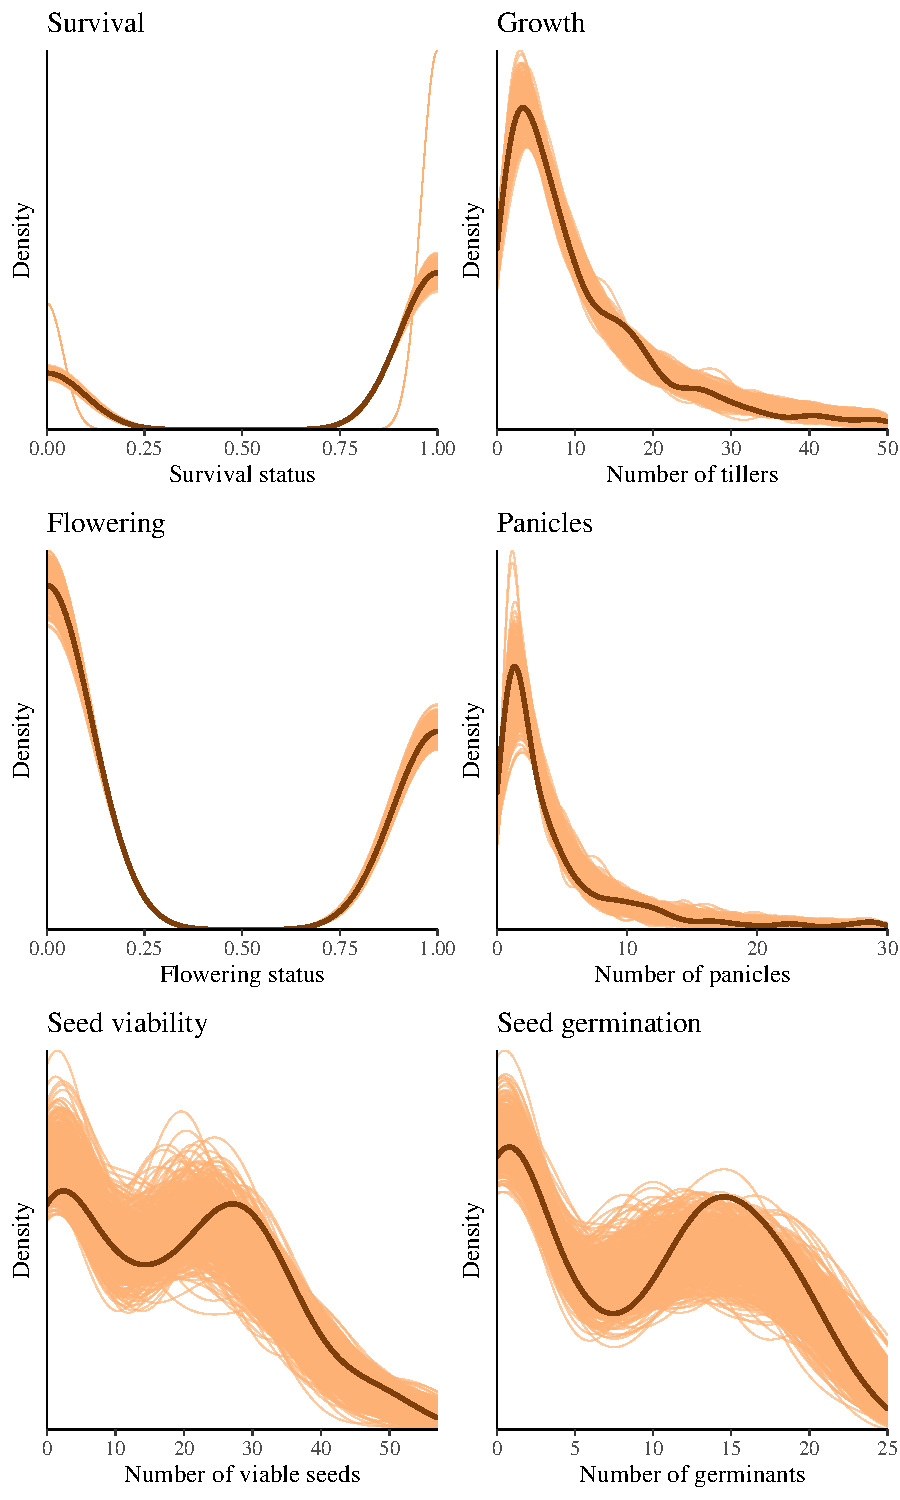
\includegraphics[width=0.75\linewidth]{PPC.pdf}
\caption{Posterior predictive checks. Consistency between real data and simulated values suggests that the fitted vital rate models accurately describes the data. Graph shows density curves for the observed data (light orange ) along with the simulated values (dark orange).}
\label{Sup:PPC}
\end{figure}
\clearpage

\begin{figure}
\centering
\includegraphics[width=\textwidth]{clim_norm_vs_weather.pdf}
\caption{Comparison of 30-year (1990-2019) climate normals and observed weather conditions at common garden sites during the 2014--15 and 2015--16 census periods. Temperature is in \degree C and precipitation is in $mm$. Colors represent sites and lines show the $y=x$ relationship.}
\label{Sup:climate_normal_weather}
\end{figure}
\clearpage


\section*{Supporting  Table}
\begin{table}[]
\centering
 \caption{\revise{Estimated coefficients for vital rates, including posterior means, 95\% credible intervals, the probability of the coefficient being greater than 0, and the probability of the coefficient being less than 0. 
 The coefficients were estimated using a Bayesian mixed-effects model.}}
\begin{tabular}{lllllll}
\toprule
\textbf{Vital rate} & \textbf{Coefficient} & \textbf{mean} & \textbf{2.50\%} & \textbf{97.50\%} & \textbf{Pr (Coeff \textgreater 0)} & \textbf{Pr (Coeff \textless  0)} \\
\midrule
Survival & size*sex & -0.153 & -0.543 & 0.250 & 0.226 & 0.774 \\
Survival & sex & -0.382 & -1.667 & 0.838 & 0.275 & 0.725 \\
Survival & pptgrow*sex & -0.317 & -1.160 & 0.553 & 0.232 & 0.768 \\
Survival & pptdorm*sex & -0.146 & -0.855 & 0.590 & 0.337 & 0.663 \\
Survival & tempgrow*sex & -0.431 & -1.292 & 0.428 & 0.168 & 0.832 \\
Survival & tempdorm*sex & -0.238 & -1.169 & 0.728 & 0.311 & 0.689 \\
Survival & tempdorm*pptdorm*sex & -0.436 & -1.135 & 0.246 & 0.108 & 0.892 \\
Survival & tempgrow*pptgrow*sex & 0.514 & -0.186 & 1.214 & 0.649 & 0.351 \\
Survival & pptgrow2*sex & 0.175 & -0.394 & 0.753 & 0.729 & 0.271 \\
Survival & pptdorm2*sex & -0.317 & -0.743 & 0.101 & 0.066 & 0.934 \\
Survival & tempgrow2*sex & 0.351 & -0.447 & 1.166 & 0.224 & 0.776 \\
Survival & tempdorm2*sex & -0.204 & -0.764 & 0.349 & 0.809 & 0.191 \\
Growth & size*sex & 0.169 & 0.017 & 0.315 & 0.983 & 0.017 \\
Growth & sex & -0.254 & -0.753 & 0.258 & 0.160 & 0.840 \\
Growth & pptgrow*sex & 0.421 & 0.070 & 0.784 & 0.992 & 0.008 \\
Growth & pptdorm*sex & -0.212 & -0.502 & 0.079 & 0.077 & 0.923 \\
Growth & tempgrow*sex & 0.176 & -0.155 & 0.486 & 0.854 & 0.146 \\
Growth & tempdorm*sex & -0.308 & -0.664 & 0.036 & 0.043 & 0.957 \\
Growth & tempdorm*pptdorm*sex & -0.158 & -0.368 & 0.044 & 0.069 & 0.931 \\
Growth & tempgrow*pptgrow*sex & -0.005 & -0.314 & 0.303 & 0.967 & 0.033 \\
Growth & pptgrow2*sex & -0.141 & -0.317 & 0.020 & 0.046 & 0.954 \\
Growth & pptdorm2*sex & -0.052 & -0.209 & 0.106 & 0.256 & 0.744 \\
Growth & tempgrow2*sex & -0.066 & -0.367 & 0.242 & 0.876 & 0.124 \\
Growth & tempdorm2*sex & 0.105 & -0.077 & 0.277 & 0.337 & 0.663 \\
Flowering & size*sex & 0.150 & -0.277 & 0.578 & 0.759 & 0.241 \\
Flowering & sex & -0.810 & -2.324 & 0.773 & 0.144 & 0.856 \\
Flowering & pptgrowsex & -0.087 & -1.158 & 0.934 & 0.439 & 0.561 \\
Flowering & pptdormsex & -0.189 & -1.052 & 0.683 & 0.339 & 0.661 \\
Flowering & tempgrowsex & -0.215 & -1.208 & 0.783 & 0.339 & 0.661 \\
Flowering & tempdormsex & -0.086 & -1.164 & 0.976 & 0.444 & 0.556 \\
Flowering & tempdorm*pptdorm*sex & -0.105 & -0.701 & 0.517 & 0.371 & 0.629 \\
Flowering & tempgrow*pptgrow*sex & -0.174 & -1.192 & 0.857 & 0.651 & 0.349 \\
Flowering & pptgrow2*sex & 0.306 & -0.214 & 0.832 & 0.869 & 0.131 \\
Flowering & pptdorm2*sex & -0.086 & -0.695 & 0.503 & 0.394 & 0.606 \\
Flowering & tempgrow2*sex & -0.348 & -1.295 & 0.545 & 0.535 & 0.465 \\
Flowering & tempdorm2*sex & 0.022 & -0.529 & 0.552 & 0.236 & 0.764 \\
Panicles & size*sex & 0.037 & -0.088 & 0.158 & 0.732 & 0.268 \\
Panicles & sex & -0.068 & -0.340 & 0.211 & 0.303 & 0.697 \\
Panicles & pptgrow*sex & -0.041 & -0.289 & 0.203 & 0.361 & 0.639 \\
Panicles & pptdorm*sex & 0.010 & -0.210 & 0.233 & 0.534 & 0.466 \\
Panicles & tempgrow*sex & 0.008 & -0.236 & 0.268 & 0.514 & 0.486 \\
Panicles & tempdorm*sex & -0.096 & -0.341 & 0.157 & 0.229 & 0.771 \\
Panicles & tempdorm*pptdorm*sex & 0.015 & -0.207 & 0.234 & 0.555 & 0.445 \\
Panicles & tempgrow*pptgrow*sex & -0.052 & -0.287 & 0.208 & 0.289 & 0.711 \\
Panicles & pptgrow2*sex & 0.059 & -0.153 & 0.264 & 0.719 & 0.281 \\
Panicles & pptdorm2*sex & 0.042 & -0.148 & 0.236 & 0.668 & 0.332 \\
Panicles & tempgrow2*sex & -0.116 & -0.370 & 0.144 & 0.173 & 0.827 \\
Panicles & tempdorm2*sex & -0.092 & -0.284 & 0.100 & 0.184 & 0.816\\
\bottomrule
\end{tabular}
\end{table}


\bibliography{Forecasting}

\end{document}
